\documentclass[10pt,a4paper]{article}
\usepackage[margin=0.5in]{geometry}
\usepackage[utf8]{inputenc}
\usepackage[english]{babel}
\usepackage{amsmath}
\usepackage{amsfonts}
\usepackage{amssymb}
\usepackage{cancel}
\usepackage{graphicx}

\title{Solid angle subtended by a tetrahedron computation}

\newcommand{\lvec}[1]{\overrightarrow{#1}}
\newcommand{\vA}{\mathbf{A}}
\newcommand{\vB}{\mathbf{B}}
\newcommand{\vC}{\mathbf{C}}
\newcommand{\vG}{\mathbf{G}}
\newcommand{\va}{\mathbf{a}}
\newcommand{\vb}{\mathbf{b}}
\newcommand{\vc}{\mathbf{c}}

\begin{document}

\maketitle


\includegraphics[scale=0.4]{tetra.png}


\section{Notations}

Let us denote, respectively:
\begin{itemize}
  \item vectors $\lvec{OA}$, $\lvec{OB}$, $\lvec{OC}$ and $\lvec{OG}$ by $\vA$, $\vB$, $\vC$ and $\vG$,
  \item vectors $\lvec{GA}$, $\lvec{GB}$ and $\lvec{GC}$ by $\va$, $\vb$, $\vc$,
  \item vector norms $\|\lvec{OA}\|$, $\|\lvec{OB}\|$ and $\|\lvec{OC}\|$ by $A$, $B$, $C$.
\end{itemize}





\section{Computation}

The solid angle $\Omega$ subtended by the triangular surface $ABC$ is given by \cite{bib:vanOos1983solid}:
\begin{equation}
  \tan \left( {\frac {1}{2}}\Omega \right)
    = \frac{ \left| \mathbf{A \ B \ C}\right| }
           { A B C
             + ( \mathbf{A} \cdot \mathbf{C} ) A
             + ( \mathbf{A} \cdot \mathbf{C} ) B
             + ( \mathbf{A} \cdot \mathbf{B} ) C
           }
  \label{eq:refFormula}
\end{equation}

where $\left| \mathbf{A \ B \ C}\right| = \mathbf{A} \cdot (\mathbf{B} \times \mathbf{C})$.



  \subsection{Numerator}

Given that $\vA = \lvec{OA} = \vG + \va$ (and resp. with $B$ and $C$), we get:
\begin{align*}
  \left| \mathbf{A \ B \ C}\right|
  & = \vA \cdot (\vB \times \vC) \\
  & = (\vG + \va) \cdot ( (\vG + \vb) \times (\vG + \vc) ) \\
  & = (\vG + \va) \cdot (  \cancel{\vG \times \vG}
                         + \vG \times \vc
                         + \vb \times \vG
                         + \vb \times \vc) \\
  & = \cancel{\vG \cdot (\vG \times \vc)}
    + \cancel{\vG \cdot (\vb \times \vG)}
    + \vG \cdot (\vb \times \vc)
    + \va \cdot (\vG \times \vc)
    + \va \cdot (\vb \times \vG)
    + \cancel{\va \cdot (\vb \times \vc)} \\
  & = \vG \cdot (\vb \times \vc)
    + \vG \cdot (\vc \times \va)
    + \vG \cdot (\va \times \vb) \\
  & = \vG \cdot \left(  \vb \times \vc
                      + \vc \times \va
                      + \va \times \vb \right)
\end{align*}

which simplifies further given that the point $G$ is the centroid of $ABC$, \textit{i.e.}
\begin{equation}
  a + b + c= 0
  \label{eq:SAcentroid}
\end{equation}

leading to
\begin{align}
  \left| \mathbf{A \ B \ C}\right|
  & = \vG \cdot \left(  \vb \times \vc
                      + \vc \times \va
                      + \va \times \vb \right)
  \nonumber \\
  & = \vG \cdot \left(  \vb \times \vc
                      + \vc \times (-\vb-\vc)
                      + (-\vb - \vc) \times \vb \right)
  \nonumber \\
  & = \vG \cdot \left(  \vb \times \vc
                      + \vc \times (-\vb)
                      + \cancel{\vc \times (-\vc)}
                      + \cancel{(-\vb) \times \vb}
                      + (-\vc) \times \vb \right)
  \nonumber \\
  & = \vG \cdot \left(3 \vb \times \vc \right) \nonumber \\
  & = 3 \vG \cdot \left( \vb \times \vc \right)
  \label{eq:SAnumeratorSimplified}
\end{align}



  \subsection{Denominator}

To help with the implementation, we will try to reduce the number of terms that need to be pre-computed by removing terms containing $a$.

First let's see the term in $A$
\begin{align}
  ( \vB \cdot \vC ) A
  & = ( \vG + \vb ) \cdot ( \vG + \vc ) A \nonumber \\
  & = ( G^2 + \vG \cdot \vb + \vG \cdot \vc + \vc \cdot \vb) A
  \label{eq:SAdenumeratorA}
\end{align}

for which there is no need for simplification. For the term in $B$, we can use eq.~\eqref{eq:SAcentroid}:
\begin{align*}
  ( \vA \cdot \vC ) B
  & = ( \vG + \va ) \cdot ( \vG + \vc ) B \\
  & = ( G^2 + \vG \cdot \vc + \va \cdot \vG + \va \cdot \vc ) B \\
  & = ( G^2 + \vG \cdot \vc + (-\vb-\vc) \cdot \vG + (-\vb-\vc) \cdot \vc ) B \\
  & = ( G^2 - \vG \cdot \vb - \vb \cdot \vc - \vc \cdot \vc ) B
\end{align*}

where the last term can be expanded, recalling that $\vc = \vC - \vG$
\begin{align*}
  \vc \cdot \vc
  & = ( \vC - \vG ) \cdot ( \vC - \vG ) \\
  & = C^2 - 2 \vG \cdot \vC + G^2 \\
  & = C^2 - 2 \vG \cdot (\vG+\vc) + G^2 \\
  & = C^2 - 2 \vG \cdot \vc - G^2 \\
\end{align*}

finally yielding
\begin{equation}
  ( \vA \cdot \vC ) B
  = ( 2 G^2 - \vG \cdot \vb + 2 \vG \cdot \vc - \vb \cdot \vc - C^2 ) B.
  \label{eq:SAdenumeratorB}
\end{equation}

Similarly, term in $C$ can be expressed as:
\begin{equation}
  ( \vA \cdot \vB ) C
  = ( 2 G^2 + 2 \vG \cdot \vb - \vG \cdot \vc - \vb \cdot \vc - B^2 ) C.
  \label{eq:SAdenumeratorC}
\end{equation}

Finally, combining eqs.~\eqref{eq:SAdenumeratorA}, \eqref{eq:SAdenumeratorB} and \eqref{eq:SAdenumeratorC}, the denominator reads:
\begin{equation}
  A B C + ( G^2 + \vG \cdot \vb + \vG \cdot \vc + \vc \cdot \vb) A
        + ( 2 G^2 - \vG \cdot \vb + 2 \vG \cdot \vc - \vb \cdot \vc - C^2 ) B
        + ( 2 G^2 + 2 \vG \cdot \vb - \vG \cdot \vc - \vb \cdot \vc - B^2 ) C
\end{equation}

\begin{equation}
  A B C + ( A + 2B + 2C ) G^2
        + ( A -  B + 2C ) \vG \cdot \vb
        + ( A + 2B -  C ) \vG \cdot \vc
        + ( A -  B -  C ) \vb \cdot \vc
        - ( B + C ) B C
  \label{eq:SAdenominatorSimplified}
\end{equation}





\section{Final formula}

The initial formula eq.~\eqref{eq:refFormula}
\begin{equation*}
  \tan \left( {\frac {1}{2}}\Omega \right)
    = \frac{ \left| \mathbf{A \ B \ C}\right| }
           { A B C
             + ( \mathbf{A} \cdot \mathbf{C} ) A
             + ( \mathbf{A} \cdot \mathbf{C} ) B
             + ( \mathbf{A} \cdot \mathbf{B} ) C
           }
\end{equation*}

can finally be rewritten by combining eqs.~\eqref{eq:SAnumeratorSimplified} and \eqref{eq:SAdenominatorSimplified} as
\begin{equation*}
  \tan \left( {\frac {1}{2}}\Omega \right)
    = \frac{ 3 \vG \cdot \left( \vb \times \vc \right) }
           { A B C + ( A + 2B + 2C ) G^2
             + ( A -  B + 2C ) \vG \cdot \vb
             + ( A + 2B -  C ) \vG \cdot \vc
             + ( A -  B -  C ) \vb \cdot \vc
             - ( B + C ) B C
           }
\end{equation*}


\bibliographystyle{plain}
\bibliography{KO_version}

\end{document}
